\documentclass[3p]{elsarticle}
\usepackage{amsmath, amsfonts, amssymb, bm, graphicx}

\title{Three dimensional low-temperature plasma simulations on adaptive, cut-cell grids}

\author[sintef]{Robert Marskar}
\ead{robert.marskar@sintef.no}
\address[sintef]{SINTEF Energy Research}

\def\diff{\ensuremath{\text{d}}}

\begin{document}
\begin{abstract}
  We present an adaptive mesh refinement (AMR) code for three-dimensional simulations of weakly ionized plasmas in the minimal plasma model. A cut-cell formalism is used for the inclusion of solid boundaries in the form of conductors and dielectrics. 
\end{abstract}
\maketitle

\section{Introduction}
A streamer is a non-thermal, weakly ionized plasma filament with a bright (i.e. radiating) head. It exists, for example, in the pre-breakdown phase of an electrical flashover where the streamer is responsible for the creation of a slightly conductive channel. Large currents may then flow between the anode and cathode, causing additional heating of the channel which is eventually short-circuited. A streamer moves due to the motion of non-Maxwellian electrons in the head, and may move with or against the electron drift direction. If a streamer moves with the electron drift direction, it contains a net negative charge in the head is called a negative streamer. Conversely, if a streamer moves \emph{opposite} to the electron drift direction, it contains a net positive charge in the head and is called a positive streamer. For a positive streamer to propagate, it must be supported by additional phenomena beyond electron impact ionization. In air, a positive streamer is believed to propagate by the production of seed electrons in front of the head which are produced by photoionization of oxygen. The photons themselves are produced by relaxation of excited $\text{N}_2$ molecules, which are in turn produced by electron impact excitation. However, it is also believed that a positive streamer can propagate through other mechanisms; such as electron detachment from a background ionization. 

The computational modelling of weakly ionized plasmas is inherently difficult due to the existence multiple length and time scales. For atmospheric air, for example, a streamer channel is surrounded by a space charge layer with a thickness in the micrometer range, while the streamer itself can propagate tens of centimeters. Typical aspect ratios up to 1000 can therefore easily be envisioned, and adaptive mesh refinement (AMR) is almost universally required for numerically resolving such phenomena, especially in three dimensions. The inclusion of internal boundary conditions inside the computational domain leads to additional complexities, and it essential that these can be resolved in a way that remain compatible with AMR. Other difficulties of a more fundamental nature are related to the treatment of the various species (neutral, ions, electrons). For the most part, neutrals and ions are close to equilibrium for weakly ionized plasmas, and the velocity distribution function (VDF) is therefore Maxwellian so that they can be treated in the continuum (i.e. fluid) approximation. This is not necessarily the case for electrons whose VDF may be far from Maxwellian and may therefore require a kinetic (i.e. particle based) treatment. Hybrid models that combine kinetic and fluid approaches are, strictly speaking, still in their infancy but are starting to gain traction in the plasma community. The stability of such methods have been a challenge due to the inherent statistical noise that is present in e.g. Direct Monte Carlo Simulations (DMCS) or Particle-In-Cell (PIC) based approaches. Methods for direct solutions of the Boltzmann equation are also being developed. The Discrete Velocity Method, for example, reduces the Boltzmann equation to a system of hyperbolic equations for a set of velocities and is therefore a direct analogue of the Discrete Ordinates Method (DOM) for the radiative transfer equation (RTE). The DVM is, strictly speaking, different from Lattice-Boltzmann methods due to the number of velocities that are included in the discretization of phase space (usually $10^3$ for DVM versus $10^1$ for LBM). Nonetheless, simplified plasma models are still of great interest because of their simplicity and their straightforward compatibility with embedded boundary conditions. 

In this paper we examine a minimal plasma model consisting of mass balance and field equations. We include embedded boundaries in the form of electrodes and dielectrics, and examine the interaction of streamers with such surfaces. 

The structure of this paper is as follows: In Sec.~\ref{sec:theory} we review the minimal plasma model. Section~\ref{sec:method}

\section{Theory}
\label{sec:theory}

In the minimal plasma model, the equations of motion that govern the evolution the plasma are the convection-diffusion-reaction (CDR) equation for the electrons, ions, and neutrals; the Poisson equation for the electrostatic field; charge balance on each point along a dielectric surface, and the radiative transfer equation (RTE) for the radiation. Here, we apply the stationary Eddington approximation for the RTE so that our model is: 
\begin{subequations}
  \begin{align}
    \label{eq:poisson}
    \nabla\cdot(\epsilon_r\nabla)\phi &= -\frac{\rho}{\epsilon_0}, \\
    \label{eq:eddington}
    \nabla\cdot\left(\frac{1}{3\mu_\gamma}\nabla\Phi_\gamma\right) - \mu\nabla\Phi_{0,\gamma} &= -S_\gamma, \\
    \label{eq:cdr}
    \frac{\partial n}{\partial t} + \nabla\cdot\left(\bm{v}_nn\right) - \nabla\cdot\left(D_n\nabla n\right) &= S_n, \\
    \label{eq:sigma}
    \frac{\partial \sigma}{\partial t} &= F_\sigma.
  \end{align}
\end{subequations}
With this notation $\phi = \phi(\bm{x},t)$ is the electric potential ($\bm{E} = -\nabla\phi$ being the electric field), $\epsilon_r = \epsilon_r(\bm{x})$ is the relative permittivity and $\rho = \rho(\bm{x},t)$ is the charge density (accounting for both volumetric and surface charges). The vacuum permittivity is $\epsilon_0 \approx 8.854\ldots\times E-12\,\text{F/m}$. 

Furthermore, $\Phi_{0,\gamma} = \Phi_{0,\gamma}(\bm{x},t)$ is the isotropic density of a photonic species $\gamma$ which propagates through the gas phase with absorption length $\mu_\gamma = \mu_\gamma(\bm{x})$. $S_\gamma = S_\gamma(\bm{x}, t)$ is a corresponding source term for the species $\gamma$. 

The number density of a particle species (negative, position, or neutral) is denoted by $n = n(\bm{x}, t)$. Each species obeys the CDR equation and propagates through the gas volume with individual advective velocities $\bm{v}_n$, and diffuse with individual diffusion coefficients $D_n = D_n$. The rate coefficients $S_n$ describe the local mass growth or decay of species. 

Lastly, $\sigma = \sigma(\bm{x}, t)$ denotes the surface density on dielectric surfaces where $F_\sigma$ is the charge into or out of the surface. 

For streamer discharges, Eqs.~\eqref{eq:poisson}-\eqref{eq:sigma} are nonlinearly coupled in several ways. Firstly, for collisional reactions of the $X + Y \rightarrow Z$, the source terms $S_Z$ can be written as $S_Z = k_{X+Y\rightarrow Z}n_Xn_Y$ which straightforwardly demonstrates a nonlinear coupling between three species. Secondly, the coupling between the species velocities and the electric field is not necessarily linear. Even in the simplest case, a constitutive relation for $\bm{v}$ can be nonlinear $\bm{E}$ or $n$. For example, for electrons, a common simplification is $\bm{v}_e = -\mu_e(\bm{E})\bm{E}$ with a nonlinear mobility $\mu_e$. Additional nonlinearities appear, of course, in the photonic coupling, the diffusive coupling, and for the charge density. However, such couplings are application-dependent, and we therefore only specify them in our numerical examples towards the end of this paper. 

\section{Numerical method}
\label{sec:method}
Extensive experimental and computational efforts have long since established that a streamer channel is a narrow, slightly conductive channel with fine spatial features. Typically, the diameter of the channel is comparable to or less than $1\,\text{mm}$ surrounded by a space charge layer that electrostatically screens it's interior. Typically, for atmospheric pressure the spatial resolution must be less than $10\,\mu\text{m}$ while domain sizes lie somewhere in the centimeter region for the model to remain valid. It is thus clear that Eqs.~\eqref{eq:poisson}-\eqref{eq:sigma} note only evolve on multiple scales, but that the fine scale moves through the domain along with the streamer. Moreover, past computational experience has shown that the Poisson solver is usually the computational bottleneck\footnote{On Cartesian grids this is not the case for Eq.~\eqref{eq:eddington} which shows must better convergence during iterative relaxation due to a dominant on-diagonal term in the discretization stencil.}. Based on these experiences, our efforts have been guided by the need for adaptive resolution, efficient remeshing, and the availability for an efficient Poisson solver. We have therefore chosen to solve Eqs.~\ref{eq:poisson}-\ref{eq:sigma} by using the Chombo library which supplies an infrastructure for parallel data structures on cut-cell Cartesian grids, as well as some templated solvers (such as geometric multigrid). The use of cut-cell introduces some additional complexity into the discretization methods, but nonetheless support the inclusion of internal boundaries inside the computational domain.

\subsection{Spatial discretization}
Here, we give a brief summary to the spatial discretization. In general, we discretize the physical domain by a set of Cartesian control volumes centered on points $\bm{i} = (i_0, \ldots, i_{\bm{D}-1})^\intercal \in \mathbb{Z}^{\bm{D}}$ where $\bm{D}$ is the dimension (typically, $D = 2$ or $D = 3$). Each control volume occupies the region $[\bm{i} - \frac{1}{2}\bm{u}\Delta x, \bm{i} + \frac{1}{2}\bm{u}\Delta x]$ where $\Delta x$ is a resolution and $\bm{u}$ is a vector whose components are all one (i.e. $\bm{u} = (1,1)^\intercal$ in 2D). Thus, a mesh $\Gamma\subset \mathbb{Z}^{\bm{D}}$ simply consists of a set of connected cells $\bm{i} \subset \Gamma$. 



\begin{figure}[ht]
    \centering
    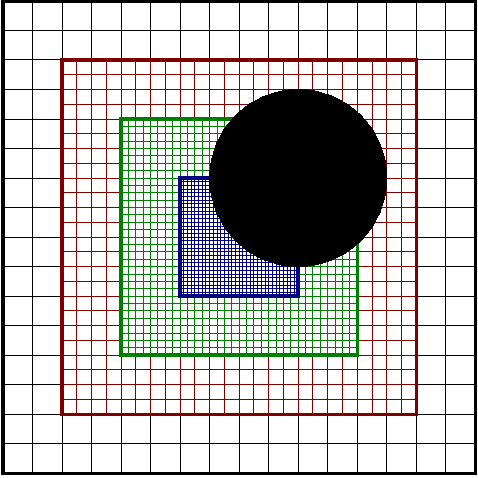
\includegraphics{./figures/amr}
    \caption{Adaptive mesh refinement}
    \label{fig:amr}
\end{figure}

Adaptive Mesh Refinement (AMR) grids are used by allowing overlapping grids with varying resolutions. We work with a set of grids $\Gamma^l$ that are nested hierarchically from the coarsest grid to the finest grid. Thus, we always require that a grid $\Gamma^l$ occupies the space between the overlapping regions of a coarser grid $\Gamma^{l-1}$ and a finer grid $\Gamma^{l+1}$. In general, the use of AMR grids for streamer simulations is advantageous due to need for regridding the solution; the use of a static mesh requires one to fully resolve the entire spatial region at the finest length scale, which leads to excessive resource requirements. Moreover, the computational overhead for remeshing a spatial region using Cartesian AMR is negligible (unlike Delaunay triangulation, for example). 

Internal boundary conditions are resolved by cutting some of the cells with a level-set function $s(\bm{x}) = 0$ which describes the boundary interface. Inside each cut-cell, the boundary is linearized so that it intersects through the cell as a line (in 2D) or plane (in 3D). Control volume faces that are cut by this surface are referred to as cut-faces, and the boundary itself is referred to as an embedded boundary (EB). 

\begin{figure}[ht]
    \centering
    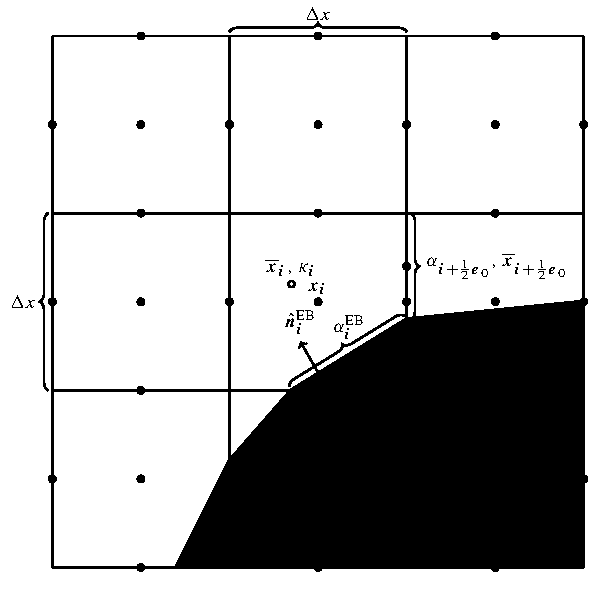
\includegraphics{./figures/spatial_discretization}
    \caption{Cut-cell discretization.}
    \label{fig:spatial_discretization}
\end{figure}

Figure~\ref{fig:spatial_discretization} shows the grid hierarchy and the cut cells in greater details. Here, a cell is denoted by it's index $\bm{i}$. We will take $\bm{x}_{\bm{i}}$ to be the cell center, and $\overline{\bm{x}}_{\bm{i}}$ to the be cell centroid. The volume fraction is $\kappa_{\bm{i}} \in [0, 1]$. Cells with $\kappa_{\bm{i}} = 0$ are denoted as \emph{covered} cells, and cells with volume fractions $0 < \kappa_{\bm{i}} < 1$ are called \emph{irregular} cells. Furthermore, cell faces are denoted by $f^\pm_d(\bm{i})$ where $\pm$ indicates the high ($+$) or low ($-$) face of the cell $\bm{i}$ in the coordinate direction $d$. A face center for face $f^\pm_d(\bm{i})$ is therefore located at $\bm{x}_{\bm{i} \pm \frac{1}{2}\mathbf{e}_d}$ where $\mathbf{e}_d$ is a unit vector in the $d$-direction. Face centroids are likewise denoted $\overline{\bm{x}}_{\bm{i} \pm \frac{1}{2}\mathbf{e}_d}$ with area fractions $\alpha_{\bm{i}\pm\frac{1}{2}\bm{e}_d}$. Finally, the EB centroid is denoted by $\overline{\bm{x}}_{\bm{i}}^{\text{EB}}$ and has an area fraction $\alpha^{\text{EB}}_{\bm{i}}$ and an outward normal vector $\bm{n}_{\bm{i}}$ . Let $V_{\bm{i}}$, $A_{\bm{i}}^{\pm, d}$, and $A_{\bm{i}}^{\text{EB}}$ denote the part of the Cartesian cell outside the boundary, the un-cut part of a face $f^{\pm}_d(\bm{i})$, and the part of the EB that intersects with the cell. Then, the above quantities are given by
\begin{subequations}
  \begin{align}
    \overline{\bm{x}}_{\bm{i}} &= \frac{1}{\Delta x^{\bm{D}}}\int_{V_{\bm{i}}}\bm{x}\diff V_{\bm{i}},\\
    \overline{\bm{x}}_{\bm{i}\pm\frac{1}{2}\bm{e}_d} &= \frac{1}{\Delta x^{\bm{D}-1}}\int_{A_{\bm{i}}^{\pm, d}}\bm{x}\diff A_{\bm{i}}^{\pm, d},\\
    \overline{\bm{x}}_{\bm{i}}^{\text{EB}} &= \frac{1}{\Delta x^{\bm{D}-1}}\int_{A_{\bm{i}}^{\text{EB}}}\bm{x}\diff A_{\bm{i}}^{\text{EB}}, \\
    \kappa_{\bm{i}} &= \frac{1}{\Delta x^{\bm{D}}}\int_{V_{\bm{i}}}\diff V_{\bm{i}},\\
    \alpha_{\bm{i}\pm\frac{1}{2}\bm{e}_d} &= \frac{1}{\Delta x^{\bm{D}-1}}\int_{A_{\bm{i}}^{\pm, d}}\bm{x}\diff A_{\bm{i}}^{\pm, d},\\
    \alpha_{\bm{i}}^{\text{EB}} &= \frac{1}{\Delta x^{\bm{D}-1}}\int_{A_{\bm{i}}^{\text{EB}}}\diff A_{\bm{i}}^{\text{EB}}, \\
    \bm{n}_{\bm{i}} &= \frac{1}{\Delta x^{\bm{D}-1}}\int_{A_{\bm{i}}^{\text{EB}}}\bm{n}\diff A_{\bm{i}}^{\text{EB}}.
  \end{align}
\end{subequations}


For brevity's sake, we will from now on omit the dependency on $\bm{i}$, and re-specify this when necessary. 

\subsection{Poisson equation}
\label{sec:poisson}
Integrating the Poisson equation over a volume $V_{\bm{i}}$ yields 
\begin{equation}
  \label{eq:poisson_operator}
  \frac{1}{\kappa_{\bm{i}}\Delta x}\left[\sum_{f\in f_d^+(\bm{i]}}\alpha_f\epsilon_fg_f^d - \sum_{f\in f_d^-(\bm{i]}}\alpha_f\epsilon_fg_f^d - \alpha_{\bm{i}}^{\text{EB}}\epsilon_{\bm{i}}^{\text{EB}}\left(\bm{g}^{\text{EB}}_{\bm{i}}\cdot\bm{n}_{\bm{i}}\right)\right] = \rho_{\bm{i}} + \sigma_{\bm{i}}
\end{equation}
This is then is discretized by using second-order approximations for the fluxes $g_f^d$ through each cell face. Note that each Cartesian face may consist of several sub-faces. For example, cells that are cut by the dielectric surface will contain two faces; one of the gas phase and one for the solid phase. This is strictly speaking not the case for faces that are cut by conducting surfaces because there is no flux passing into the volume through the part of the face that lies within the conductor. Note also that in Eq.~\ref{eq:poisson_operator}, the embedded boundary is only the conductor surfaces. The contribution of the EB fluxes for the dielectric are contained entirely within $\sigma_{\bm{i}}$, thus avoid the need for specialized boundary condition stencils for such cells. 

For un-cut faces we discretize using
\begin{equation}
  g_f^d = \frac{1}{\Delta x}\left(\phi_{\bm{i}^+}-\phi_{\bm{i}^-}\right),
\end{equation}
where $\bm{i}^\pm$ denotes the control volumes on the high ($+$) and low ($-$) sides. In order to maintain a second order scheme, cut-face fluxes are interpolated to their respective centroids. For example, for a Cartesian face which is cut by the dielectric, the flux through the face is $F = \alpha_1\epsilon_1\overline{g}_{f_1} + \alpha_2\epsilon_2\overline{g}_{f_2}$ where the subscripts $1,2$ denote the dielectric and gas phases, respectively. The two centroid fluxes $\overline{g}_{f_{1,2}}$ are obtained by interpolating cell-centered fluxes to the respective centroids. 

\subsubsection{Multigrid solver}
The discretized Poisson equation is solved by embedding it in a geometric multigrid solver in residual-correction form. Multigrid involves iterative relaxation (in our case, Gauss-Seidel relaxation) on progressively coarsened grids and is compatible with AMR. On the coarsest level, the discretized system is solved directly with a biconjugate gradient stabilized method. For our applications, we have found that a $V$-cycle type multigrid is sufficient (although we have other types of multigrid available). Typically, better convergence for each cycle is achieved the further one coarsens; for domains without embedded boundaries one may coarsen up to a level where the domain only consists of two cells in one of the coordinate direction. However, for embedded boundary applications the convergence rate is usually harmed by coarsening too far because the coarsened stencils near embedded boundary may no longer be a good approximation of the finer stencils. Moreover, coarsening may also lead to geometrical under-resolution. We avoid both of these issues by dropping to the bottom level before they manifest. 

\subsubsection{Boundary conditions}
For the Poisson equation we use either Dirichlet or Neumann boundary conditions on the domain edges, and Dirichlet on the conductors. The quasi-boundary condition for the dielectrics is implicitly contained in our discretization of the Poisson operator as discussed above. Neumann boundary conditions are straightforward to implement since they specify the boundary flux directly, whereas Dirichlet is slightly more involved. To compute Dirichlet boundary conditions we use the Johansen-Colella method by casting a ray from the EB centroid along the EB normal into the computational domain. In two dimensions, this ray will cross a coordinate line (plane in 3D) connecting two cell-centers, and the value at this point may be used to approximate the derivative $\partial_n\phi$ on the EB centroid by straightforward polynomial interpolation and differentiation. In practice, we use a second order stencil if we can, but we remark that even with a first order stencil the schme is second order due to the residual-correction form of the multigrid solver. 

Cases may arise where a stencil cannot be computed in the above form. This may occur, for example, if the cut-cell lies at the boundary of a patch. In such cases we always drop to a first order least squares approximation for the normal derivative. 

\subsection{Transport equations}
Equation~\eqref{eq:cdr} is discretized in space by using a second order Godunov method. 

\subsubsection{Hybrid divergence}


\subsection{Photon transport equation}

\subsection{Temporal discretization}

\section{Results}

\section{Conclusions}

\section*{Acknowledgements}
This work was financially supported by the Norwegian Research Council, ABB Skien, and ABB CRC. The author expresses his gratitude to D. T. Graves for help regarding multigrid and Godunov methods, and S. Pancheshnyi for fruitful discussions regarding plasma kinetics in air. 

\end{document}
